\documentclass[a4paper, 11pt]{article}
\usepackage{comment} % enables the use of multi-line comments (\ifx \fi) 
\usepackage[top = 0.5in, bottom=0.5in]{geometry}
\usepackage{color, listings, graphicx,float, booktabs, tabularx, multirow, amsmath}
\usepackage[colorlinks=true, urlcolor=blue]{hyperref}
%\geometry{margin=0.5in}

\definecolor{codegreen}{rgb}{0,0.6,0}
\definecolor{codegray}{rgb}{0.5,0.5,0.5}
\definecolor{codepurple}{rgb}{0.58,0,0.82}
\definecolor{backcolour}{rgb}{0.97,0.97,0.97}
 
\lstdefinestyle{mystyle}{
    backgroundcolor=\color{backcolour},   
    basicstyle=\footnotesize,
    breakatwhitespace=false,         
    breaklines=true,                 
    captionpos=b,                    
    keepspaces=true,                 
%    numbers=left,                    
%    numbersep=5pt,                  
    showspaces=false,                
    showstringspaces=false,
    showtabs=false,                  
    tabsize=2
}
 
\lstset{style=mystyle}
\begin{document}
\graphicspath{{./figures/}}
\noindent
\large\textbf{Final Project: Exploratory Analysis} \\
\normalsize Group Members:\\ 
Brooke Barrett, Bobbi Benson, Beckett Cromer, \\
Bill Gilronan, Dan Johnson, Kyle Salitrik \hfill
\vspace{-1em}

%%%%%%%%%%%%%%%%%%%%%%%%%%%%%%%%%%%%%%%%%%%%%%%%%%%%%%%%%%%%%%%%%%%%
%%% SECTION: Data Exploration
%%%%%%%%%%%%%%%%%%%%%%%%%%%%%%%%%%%%%%%%%%%%%%%%%%%%%%%%%%%%%%%%%%%%
\section*{Data Set Introduction}
The data being investigated concerns the performance statistics, salaries, free agency and arbitration in the 1991-1992 season and contains 337 total observations. The data was obtained from an online repository and has been cited from the following sources: CNN Sports Illustrated, Sacramento Bee, and the New York Times. The following variables are included in the data with units in parentheses:
\begin{itemize}
	\setlength\itemsep{0em}
	\item Salary (Thousands of Dollars)
	\item Batting Average (\%)
	\item On-base Percentage or OBP (\%)
	\item Counts of: Runs, Hits, Doubles, Triples, Home Runs, runs batted in or RBI, Walks, Strike-outs, Stolen Bases, and Errors
	\item Categorical Indication of: "free agency eligibility", "free agent in 1991/2", "arbitration eligibility", and "arbitration in 1991/2"
	\item Player's name
\end{itemize}
\vspace{-1em}
\subsection*{Research Questions}
The following questions will be explored:
\begin{itemize}
	\setlength\itemsep{0em}
	\item Is OBP a good prediction of salary?
	\item Does using the individual predictors that comprise OBP create a stronger model?
	\item How well does our model handle predicting actual salaries?
\end{itemize}

The models below will be used to conduct our tests on the stated questions.
\vspace{-1cm}
\begin{center}
	\begin{align*}
		\text{Singles}=           & \text{Hits}-\text{Doubles}-\text{Triples}-\text{HomeRuns}                                                           \\
		\text{Salary}_{OBP}=      & \beta_0 + \beta_1\text{Runs} + \beta_2\text{Strike-outs} + \beta_3\text{StolenBases} + \beta_4\text{OBP} + \epsilon \\
		\text{Salary}_{Expanded}= & \beta_0 + \beta_1\text{Runs} + \beta_2\text{Strike-outs} + \beta_3\text{StolenBases} + \beta_4\text{Singles}        \\
		                          & + \beta_5\text{Doubles} + \beta_5\text{Triples} + \beta_6\text{HomeRuns} + \beta_7\text{Walks} + \epsilon           
	\end{align*}
\end{center}

%%%%%%%%%%%%%%%%%%%%%%%%%%%%%%%%%%%%%%%%%%%%%%%%%%%%%%%%%%%%%%%%%%%%
%%% SECTION: CODE APPENDIX
%%%%%%%%%%%%%%%%%%%%%%%%%%%%%%%%%%%%%%%%%%%%%%%%%%%%%%%%%%%%%%%%%%%%
\section*{Data Exploration}

\subsection*{Summary}
Below is the summary of our data using R.
\vspace{-1em}
\begin{figure}[H]
	\centering
	\caption{R Summary Output}
	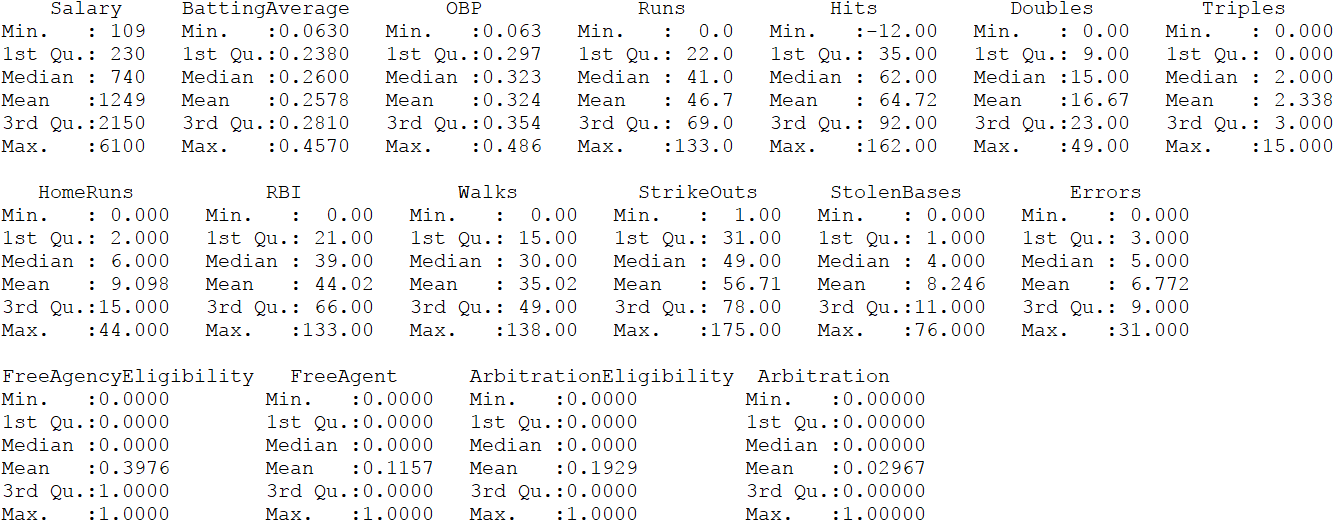
\includegraphics[width=\textwidth]{summary.png}
\end{figure}

\subsection*{Errors}
Looking into the summary statistics, it can be observed that the minimum of Hits is equal to -12, which indicates a likely error. This data point corresponds to Bo Jackson records. This player's observations will be removed from the data set due to this finding.

\subsection*{Correlations}
The following values were obtained for the correlation between the variables.
\vspace{-1em}
\begin{figure}[H]
	\centering
	\caption{R Correlation Matrix Output}
	\centerline{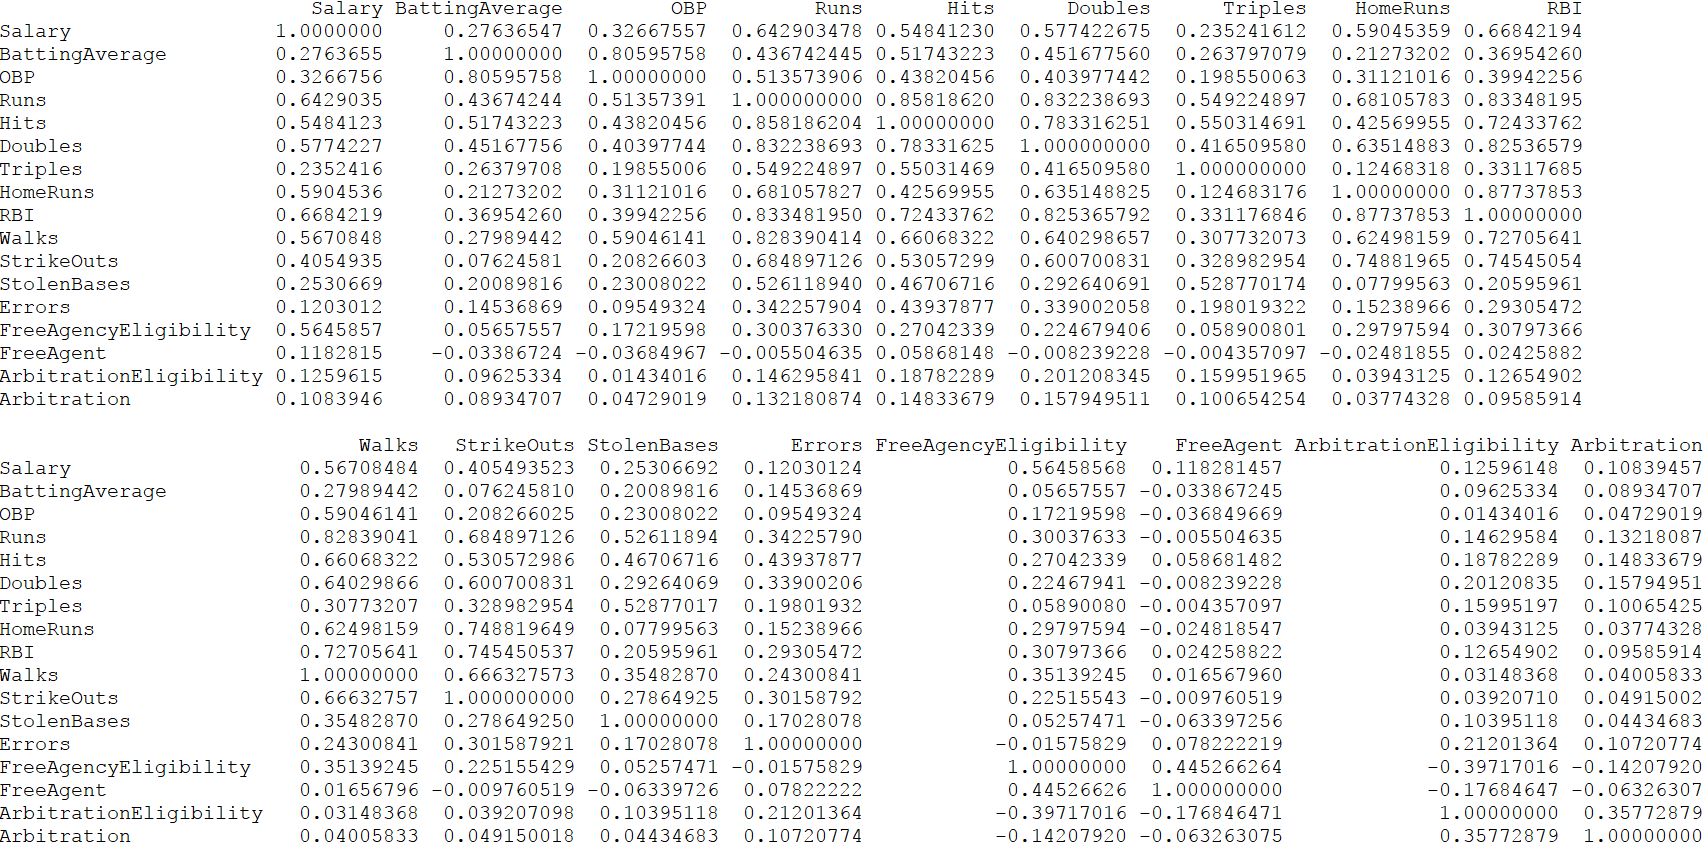
\includegraphics[width=7in]{correlation.png}}
\end{figure}

\subsection*{Scatter Plots}
The first figure includes the scatter plots that concern the $Salary_{OBP}$ model and the second includes the scatter plots introduced in the $Salary_{Expanded}$ model.
\vspace{-1em}
\begin{figure}[H]
	\centering
	\caption{OBP Model Scatter Plots}
	\centerline{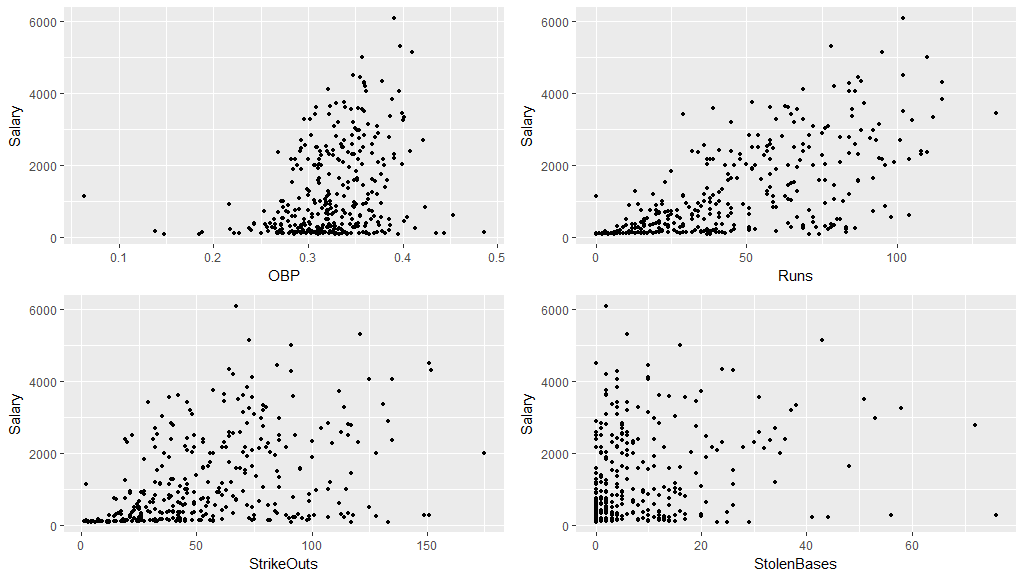
\includegraphics[width=\textwidth]{scatter_salary.png}}
\end{figure}
\vspace{-1em}
\begin{figure}[H]
	\centering
	\caption{Extended Model Scatter Plots}
	\centerline{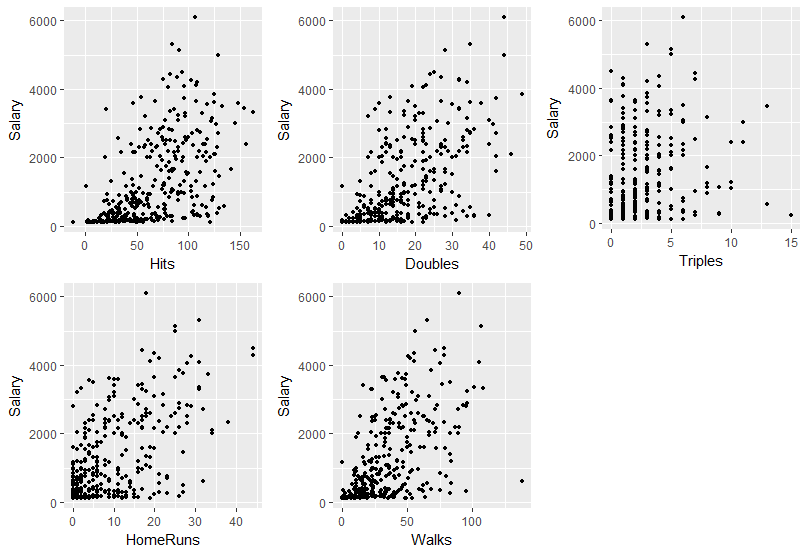
\includegraphics[width=\textwidth]{scatter_salary_expanded.png}}
\end{figure}

\subsection*{Data Distribution}
From our data distribution one can see non-normal data will be an issue to deal with.
\vspace{-1em}
\begin{figure}[H]
	\centering
	\caption{R Correlation Matrix Output}
	\centerline{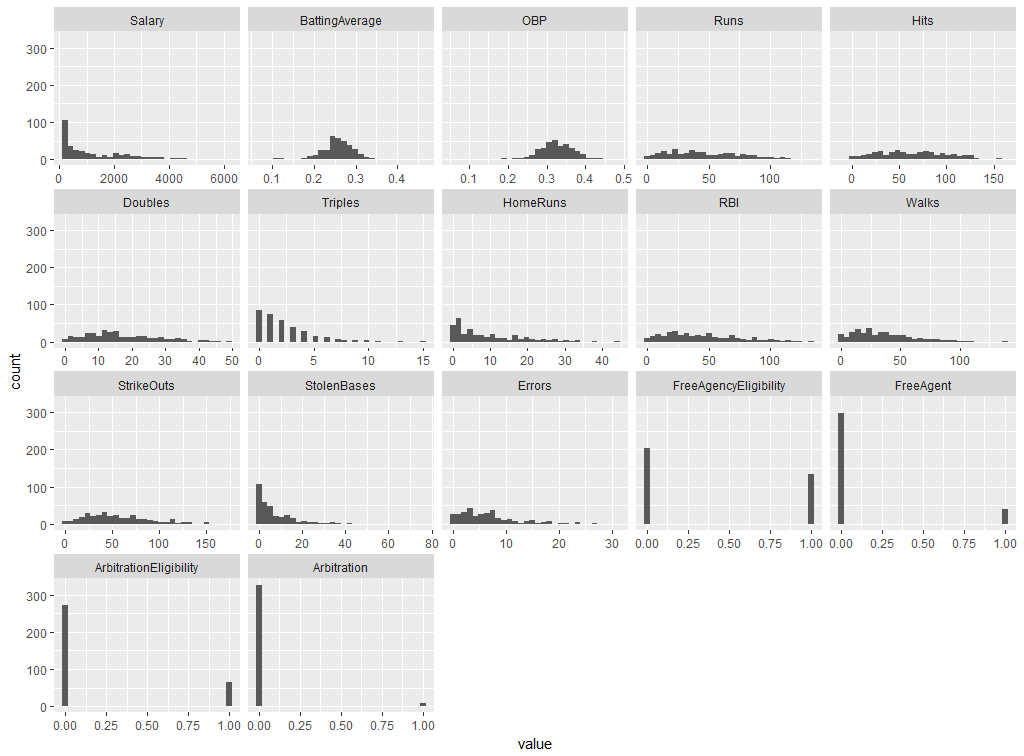
\includegraphics[width=7in]{data_distribution.png}}
\end{figure}
\end{document}